% The CONCLUSIONS.md ledger: how a claim moves, and how the ledger reaches the agent.
% Colours come from src/styles/palette.json via the generated ../_palette.tex (npm run tokens).
% Shared house style for the TikZ diagrams. render.sh defines \theme (light|dark) before \input.
\documentclass{article}
\usepackage{fontspec}
\usepackage{tikz}
\usepackage{fontawesome5}
\usetikzlibrary{positioning,calc,arrows.meta,fit,backgrounds}
\setmainfont{CrimsonPro}[Path=\fontdir, Extension=.ttf, UprightFont=*, ItalicFont=*-Italic, UprightFeatures={RawFeature={+wght=400}}, ItalicFeatures={RawFeature={+wght=400}}, BoldFont=*, BoldFeatures={RawFeature={+wght=600}}, Scale=1.08]
\setmonofont{JetBrainsMono}[Path=\fontdir, Extension=.ttf, Scale=0.86]
\newfontfamily\kickerfont{JetBrainsMono}[Path=\fontdir, Extension=.ttf, Scale=0.72, LetterSpace=12]
% GENERATED from src/styles/palette.json by scripts/tokens/build.mjs. Do not edit; run `npm run tokens`.
\def\darktheme{dark}
\ifx\theme\darktheme
  \definecolor{ink}{HTML}{EFEFE8}
  \definecolor{muted}{HTML}{A0A09A}
  \definecolor{paper}{HTML}{1B1B19}
  \definecolor{accent}{HTML}{5FE08F}
  \definecolor{accentfill}{HTML}{173322}
  \definecolor{oxide}{HTML}{FF6A4D}
\else
  \definecolor{ink}{HTML}{111111}
  \definecolor{muted}{HTML}{4A4A4A}
  \definecolor{paper}{HTML}{FFFFF8}
  \definecolor{accent}{HTML}{1F7A45}
  \definecolor{accentfill}{HTML}{E6F1EA}
  \definecolor{oxide}{HTML}{C8361C}
\fi

\tikzset{
  every picture/.style={line cap=round, line join=round, font=\normalsize, text=ink},
  card/.style={draw=ink!70!paper, line width=0.6pt, fill=paper, rounded corners=3pt, align=left,
               text width=#1, inner xsep=7pt, inner ysep=5.5pt, anchor=north west},
  card/.default=3.9cm,
  hot/.style={card=#1, draw=accent, line width=1.1pt, fill=accentfill},
  hot/.default=3.9cm,
  ghost/.style={card=#1, draw=muted!80!paper, dashed, fill=none, text=muted},
  ghost/.default=3.9cm,
  panel/.style={draw=muted!45!paper, line width=0.5pt, rounded corners=5pt, inner sep=9pt},
  hotpanel/.style={panel, draw=accent!75!paper, line width=0.9pt},
  line/.style={-{Stealth[length=5pt,width=4.2pt]}, line width=0.7pt, draw=ink!70!paper},
  hotline/.style={line, draw=accent, line width=1pt},
  ghostline/.style={line, draw=muted!80!paper, dashed},
  badline/.style={line, draw=oxide, line width=1pt},
  lbl/.style={font=\small\itshape, text=muted, inner sep=2.5pt},
  head/.style={font=\itshape, text=muted, anchor=south west, inner sep=0pt, align=left},
  warm/.style={card=#1, draw=accent!60!paper, fill=accentfill!50!paper},
  warm/.default=3.9cm,
}
\newcommand{\kicker}[1]{{\kickerfont\MakeUppercase{#1}}}
\newcommand{\ico}[1]{\makebox[1.25em][l]{#1}}
\newcommand{\cardtext}[2]{{\ttfamily #1}\\[1pt]{\small\itshape\color{muted}#2}}
% Crop the page to the picture: typeset it into a box and ship that box as the page.
\newcommand{\diagram}[1]{%
  \setbox0\hbox{#1}%
  \pagewidth=\dimexpr\wd0+8pt\relax \pageheight=\dimexpr\ht0+\dp0+8pt\relax
  \hoffset=-1in \voffset=-1in
  \shipout\vbox{\kern4pt\hbox{\kern4pt\box0}}}

\begin{document}
\diagram{\begin{tikzpicture}[x=1cm,y=1cm]
  \def\tw{4.6cm}
  \node[head, anchor=south west] (h) at (0,0.3) {\kicker{the ledger}\\[3pt]{\upshape\ttfamily\color{ink}\faIcon{file-alt}\ \ CONCLUSIONS.md}};
  \node[card=\tw] (open) at (0,0) {\cardtext{\faIcon{question-circle}\ \ Open}{still being tested}};
  \node[hot=\tw, below=0.85cm of open.south west, anchor=north west] (est) {\cardtext{\faIcon{check-circle}\ \ Established}{the claim, its evidence, a date}};
  \node[ghost=\tw, below=0.85cm of est.south west, anchor=north west] (ret) {\cardtext{\faIcon{times-circle}\ \ Retracted}{the claim, and why it was wrong}};
  \draw[hotline] ($(open.south west)+(0.45,0)$) -- node[lbl, text=accent, right] {verified} ($(est.north west)+(0.45,0)$);
  \draw[ghostline] ($(est.south west)+(0.45,0)$) -- node[lbl, right] {overturned by evidence} ($(ret.north west)+(0.45,0)$);
  \begin{scope}[on background layer]
    \node[hotpanel, fit={(h) (open) (ret)}] (L) {};
  \end{scope}
  \node[card=\tw, anchor=north west] (turn) at ($(ret.south west)+(0,-1.55)$) {\cardtext{\faIcon{comment-dots}\ \ every prompt}{the whole ledger, attached to it}};
  \draw[hotline] (L.south -| turn.north) -- node[lbl, text=accent, right, align=left] {a hook pastes it in,\\ every turn} (turn.north);
\end{tikzpicture}}
\end{document}
